\message{ !name(paper.tex)}%  article.tex (Version 3.3, released 19 January 2008)
%  Article to demonstrate format for SPIE Proceedings
%  Special instructions are included in this file after the
%  symbol %>>>>
%  Numerous commands are commented out, but included to show how
%  to effect various options, e.g., to print page numbers, etc.
%  This LaTeX source file is composed for LaTeX2e.

%  The following commands have been added in the SPIE class 
%  file (spie.cls) and will not be understood in other classes:
%  \supit{}, \authorinfo{}, \skiplinehalf, \keywords{}
%  The bibliography style file is called spiebib.bst, 
%  which replaces the standard style unstr.bst.  

\documentclass[]{spie}  %>>> use for US letter paper
%%\documentclass[a4paper]{spie}  %>>> use this instead for A4 paper
%%\documentclass[nocompress]{spie}  %>>> to avoid compression of citations
%% \addtolength{\voffset}{9mm}   %>>> moves text field down
%% \renewcommand{\baselinestretch}{1.65}   %>>> 1.65 for double spacing, 1.25 for 1.5 spacing 
%  The following command loads a graphics package to include images 
%  in the document. It may be necessary to specify a DVI driver option,
%  e.g., [dvips], but that may be inappropriate for some LaTeX 
%  installations. 
\usepackage{graphicx}
\usepackage{subfig}
\usepackage{amsmath}
\usepackage{amssymb}
\usepackage{hyperref}

\title{Texture mapping 3D planar models of indoor environments with noisy camera poses} 

%>>>> The author is responsible for formatting the 
%  author list and their institutions.  Use  \skiplinehalf 
%  to separate author list from addresses and between each address.
%  The correspondence between each author and his/her address
%  can be indicated with a superscript in italics, 
%  which is easily obtained with \supit{}.

\author{Peter Cheng, Michael Anderson, Stewart He, Avideh Zakhor
\skiplinehalf
University of California, Berkeley\\
}

 

%%%%%%%%%%%%%%%%%%%%%%%%%%%%%%%%%%%%%%%%%%%%%%%%%%%%%%%%%%%%% 
%>>>> uncomment following for page numbers
% \pagestyle{plain}    
%>>>> uncomment following to start page numbering at 301 
%\setcounter{page}{301} 
 
\begin{document}

\message{ !name(paper.tex) !offset(80) }
\section{Simple Texture Mapping}
\label{sec:simpleTextureMapping}

The geometry of the texture mapping process for a plane is shown in
Figure \ref{fig:projection}.  As described earlier, we are provided
with a set of $M$ images to texture the target plane. Each image has a
camera matrix $P_i$ for $i=1..M$, which translates a 3D point in the
world coordinate system to a 2D point or pixel in image $i$'s
coordinates. A camera matrix $P_i$ is composed of the camera's
intrinsic parameters, such as focal length and image center, as well
as extrinsic parameters which specify the rotation and translation of
the camera's position in 3D world coordinates at the time that image
$i$ is taken. These extrinsic parameters are determined by the
backpack hardware and localization algorithms \cite{chen2010indoor,
  liu2010indoor, kua2012loopclosure} and are quite noisy.

Because our backpack system takes photos at a rate of 5 Hz, thousands
of images are available for texturing each surface in our model. Our
goal in designing a texture mapping process is to decide which of
these images should be used, and where their contents should map onto
the texture, in order to minimize any visual discontinuities or seams
that would suggest that the plane's final texture is not composed of a
single continuous image.

\begin{figure}[ht]
  \begin{minipage}[b]{0.45\linewidth}
  \centering
  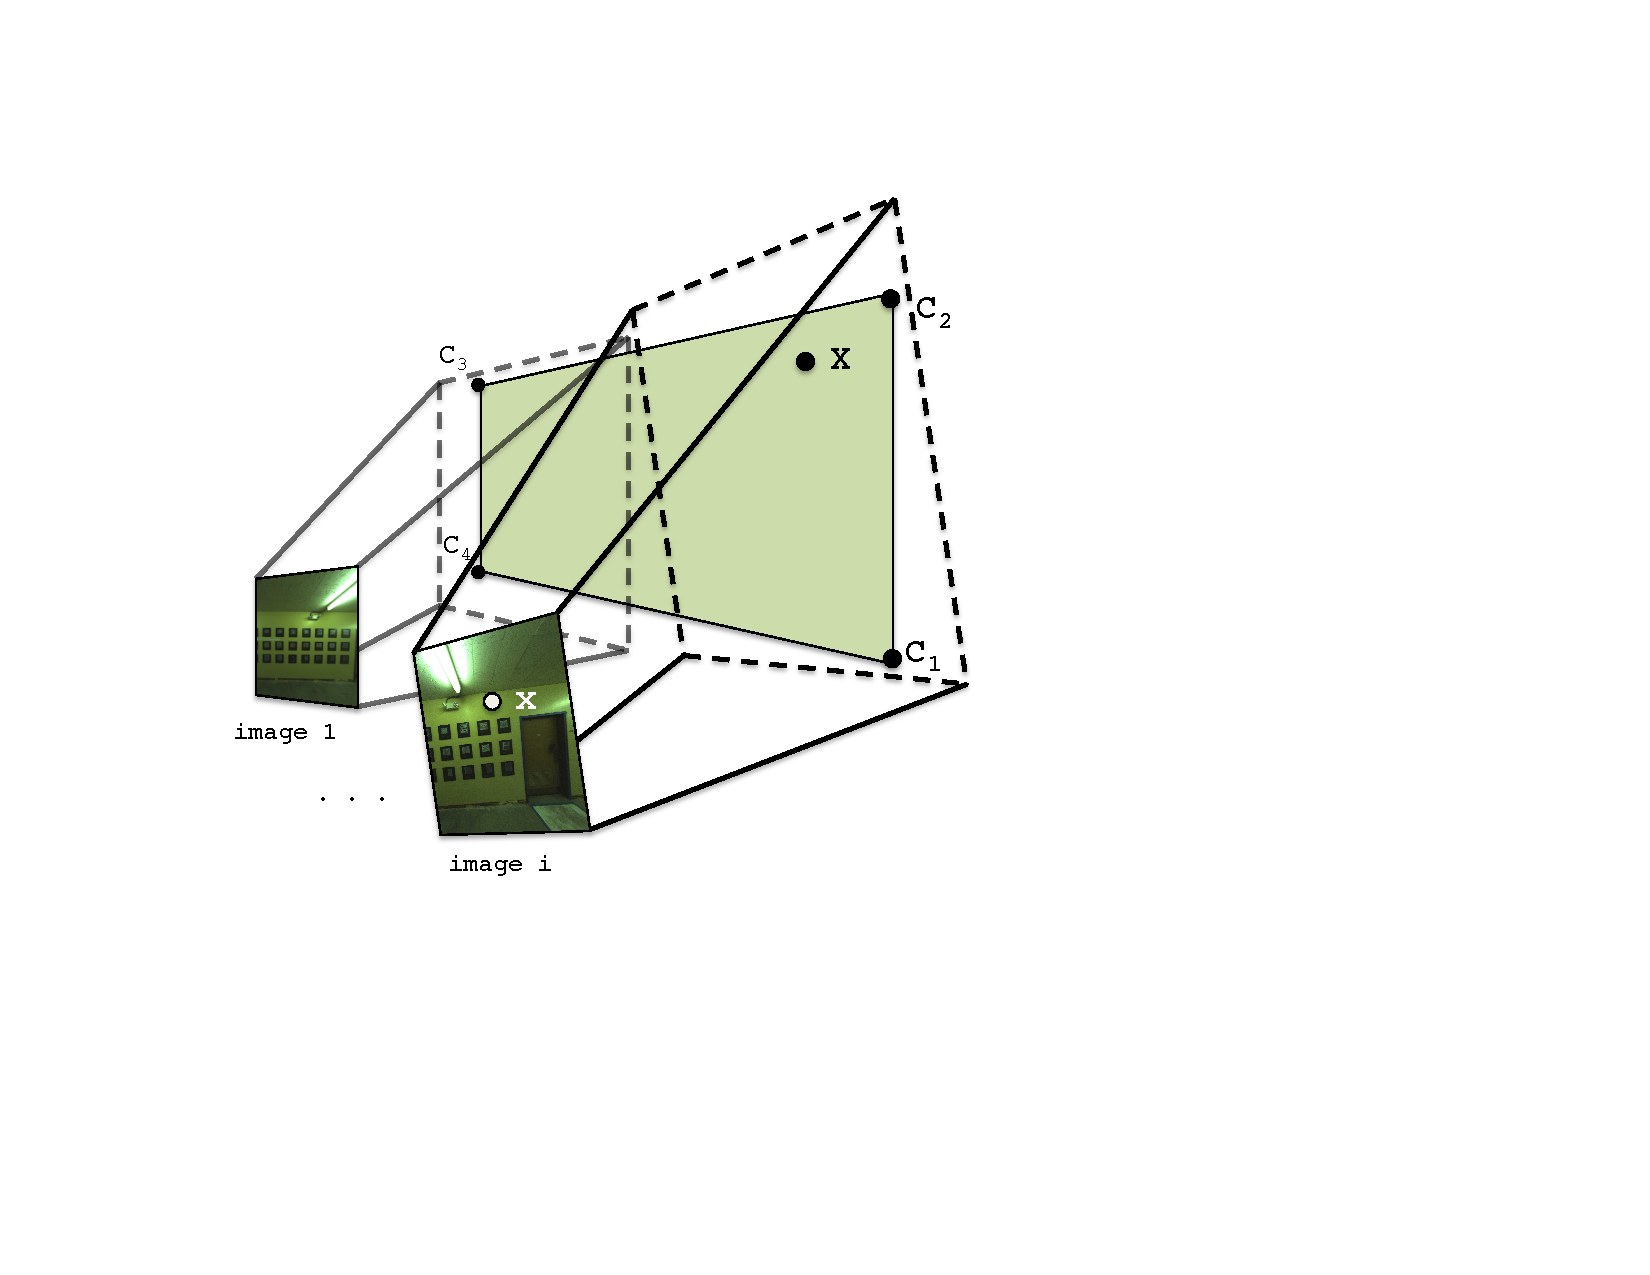
\includegraphics[height=2in]{Projection.pdf}
  \caption{Planes are specified in 3D space by four corners $C_1$ to
    $C_4$. Images are related to each plane through the camera matrics
    $P_{1..m}$. }
  \label{fig:projection}
  \end{minipage}
  \hspace{0.5cm}
  \begin{minipage}[b]{0.45\linewidth}
  \centering
  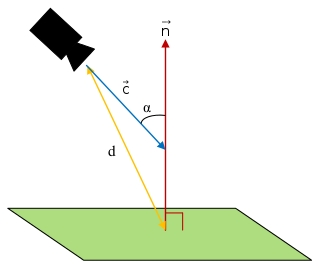
\includegraphics[height=1.5in]{scoringFunction.jpg}
  \caption{We minimize camera angle $\alpha$ and distance $d$ by
    maximizing the scoring function $\frac{1}{d} (-1 \cdot \vec{c})
    \cdot \vec{n}$}
  \label{fig:scoringFunction}
  \end{minipage}
\end{figure}


\subsection{Tile-based Texture Mapping}
\label{sec:tileBasedMapping}
Ignoring the fact that the camera matrices $P_{1..M}$ are inaccurate,
we can texture the plane by discretizing it into small square tiles,
in our case 5 pixels across, and choosing an image to texture each
tile.

We choose to work with rectangular units to ensure that borders
between any two distinct images in the final texture are either
horizontal or vertical. Since most strong environmental features
inside buildings are horizontal or vertical, any visible seams in our
texture intersect them minimally and are less noticeable.

In order to select an image for texturing a tile $t$, we must first
gather a list of candidate images that contain all four of its
corners, which we can quickly check by projecting $t$ into each image
using the $P_i$ camera matrices. Furthermore, each candidate image
must have been taken at a time when its camera had a clear
line-of-sight to $t$, which can be calculated using standard
ray-polygon intersection tests between the camera location, $t$, and
every other plane \cite{rayintersection}.

Once we have a list of candidate images for $t$, we define a scoring
function in order to objectively select the best image for texturing
$t$. Since camera pose errors compound over distance, we wish to
minimize the distance between cameras and the surfaces they
texture. Additionally, we desire images that are projected
perpendicularly onto the plane, maximizing the resolution and amount
of useful texture available in their projections, as well as
minimizing any parallax effects due to real-world geometry not
accurately represented by our digital model. In other words, we wish
to minimize the angle between the tile's normal vector and the camera
axis for images selected for texture mapping. These two criteria can
be met by maximizing the function $\frac{1}{d} (-1 \cdot \vec{c})
\cdot \vec{n}$ as shown in Figure
\ref{fig:scoringFunction}. Specifically, $d$ is the distance between
the centers of a camera and a tile, and $\vec{n}$ and $\vec{c}$ are
the directions of the plane's normal and the camera axis respectively.


\begin{figure}
  \centering 
  \subfloat[][]{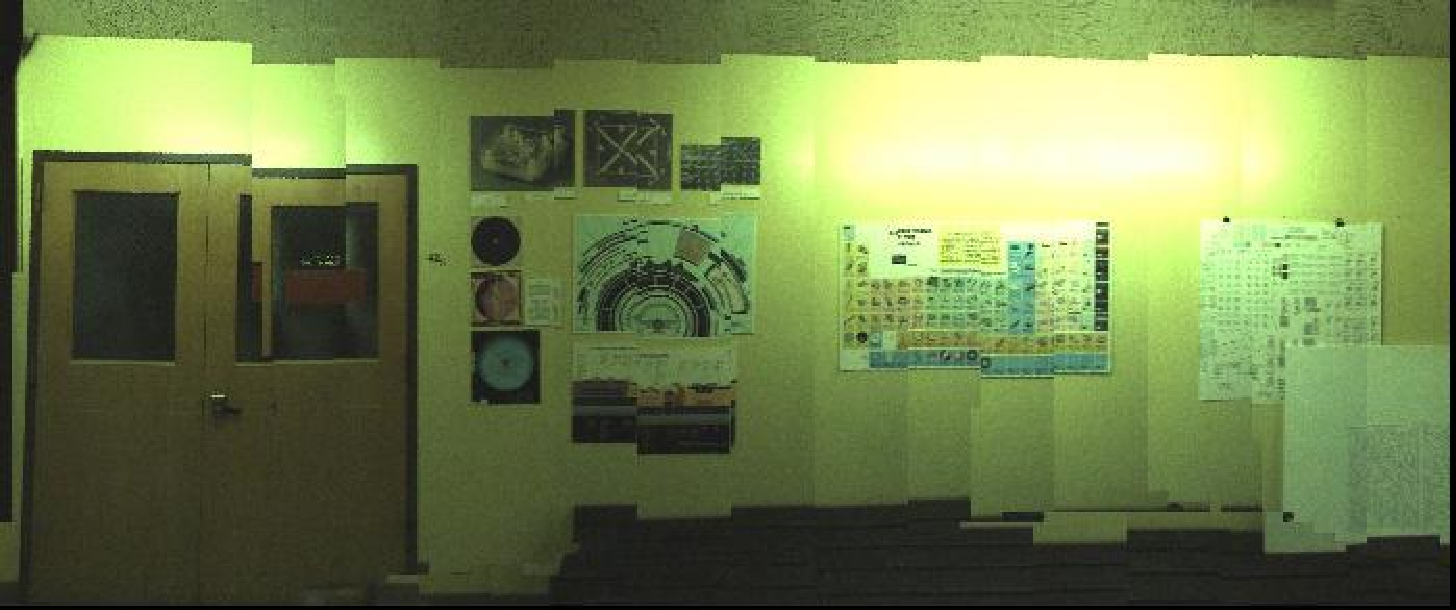
\includegraphics[width=3in, height=0.97in]{wall2_naive.pdf}}
  \subfloat[][]{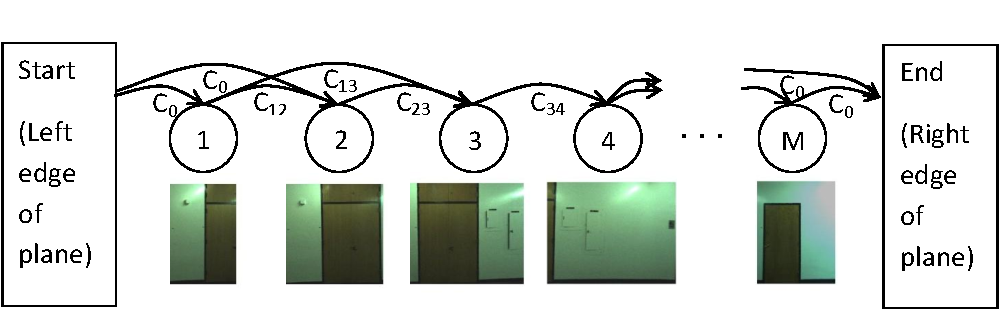
\includegraphics[width=3in, height=0.97in]{wall2_naive_shift.pdf}}

  \centering
  \subfloat[][]{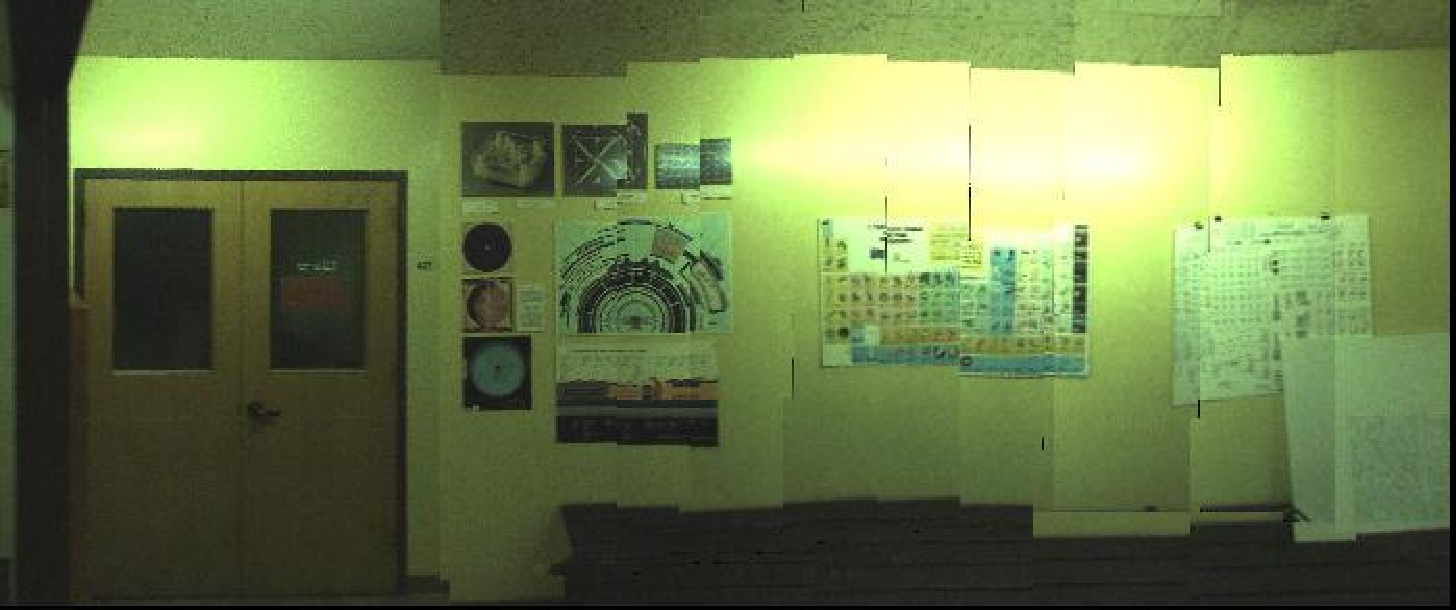
\includegraphics[width=3in, height=0.97in]{wall2_cache_shift.pdf}}
  \subfloat[][]{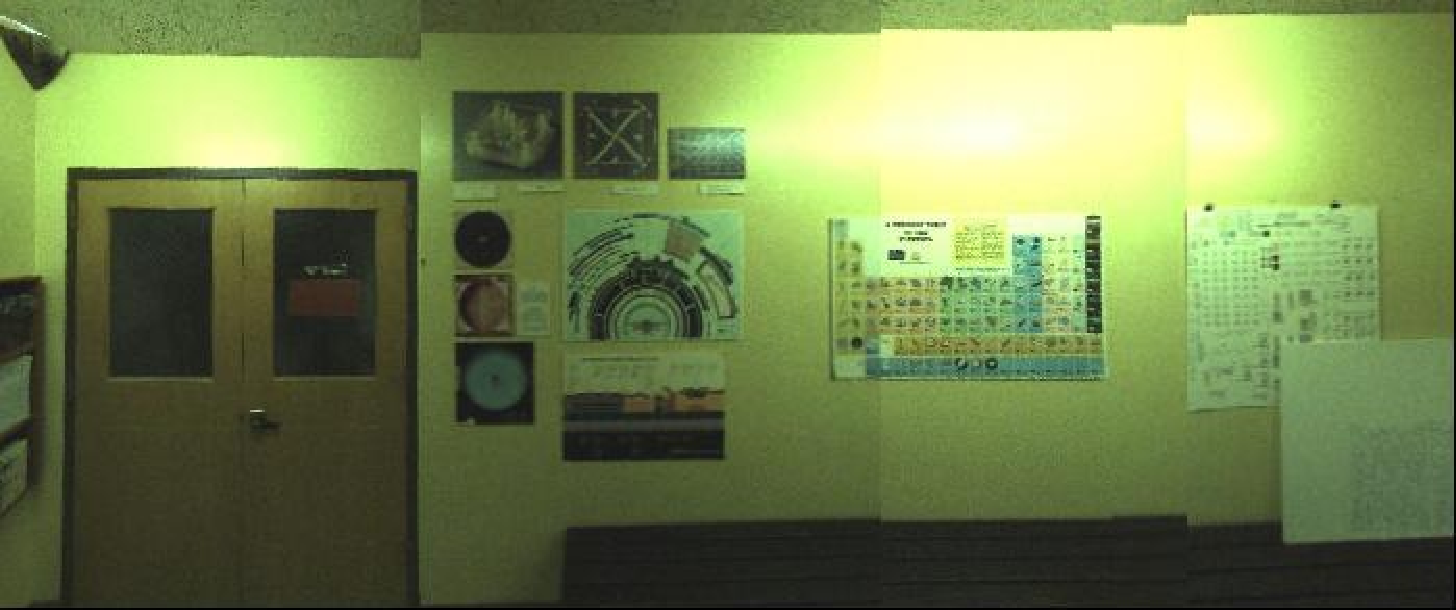
\includegraphics[width=3in, height=0.97in]{wall2_shortest_shift.pdf}}

  \centering 
  \subfloat[][]{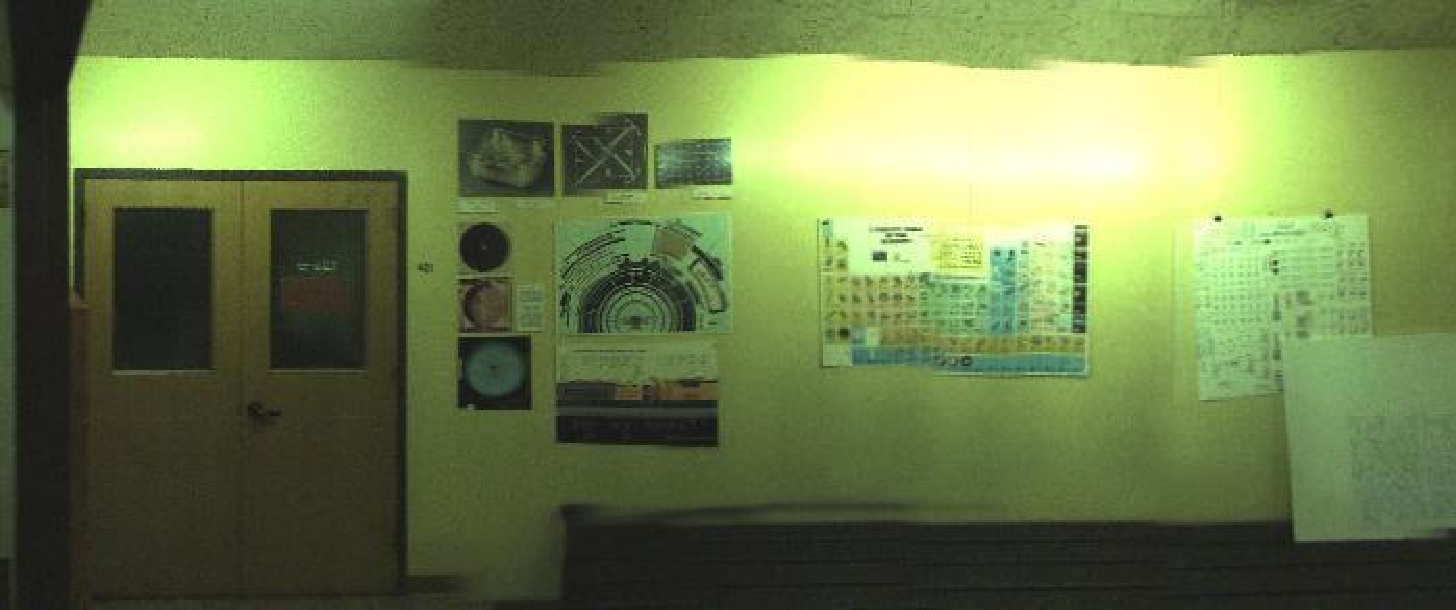
\includegraphics[width=3in, height=0.97in]{wall2_cache_shift_blend.pdf}}
  \subfloat[][]{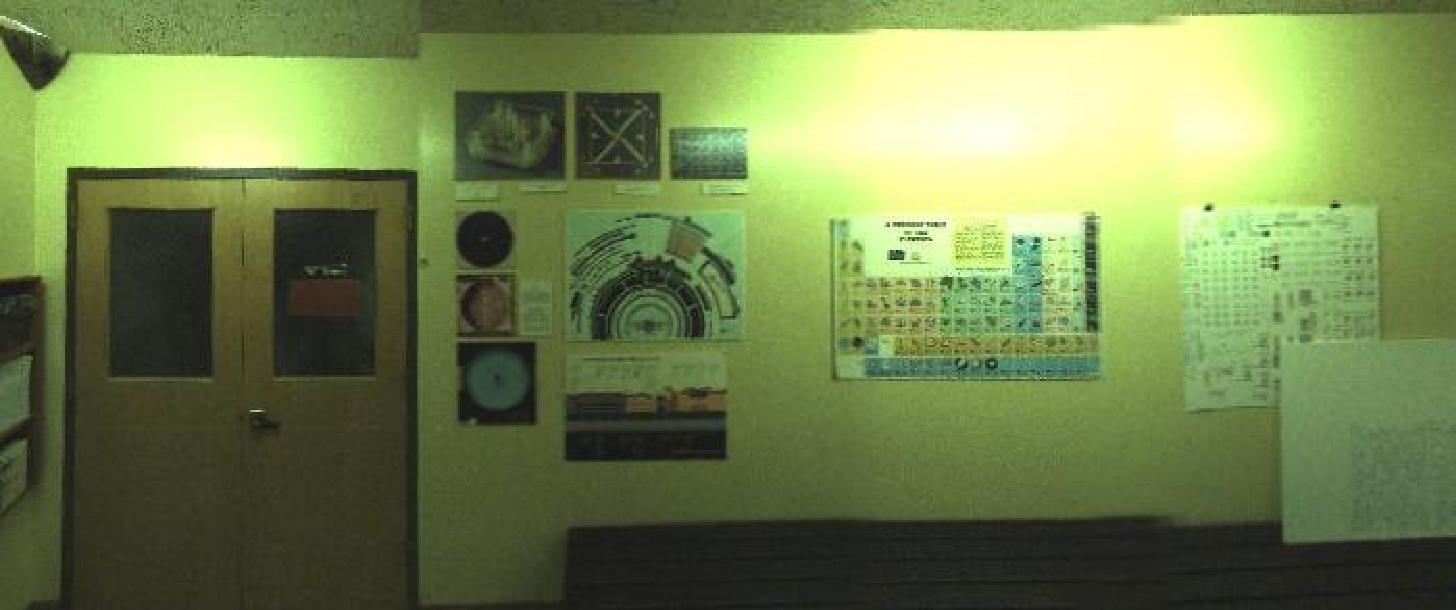
\includegraphics[width=3in, height=0.97in]{wall2_shortest_shift_blend.pdf}}
  \caption{(a) Tile-based texturing. (b) Tile-based texturing after
    image alignment. (c) Tile-based texturing after image alignment
    with caching. (d) Shortest path texturing after image
    alignment). (e) Same as (c) with blending. (f) Same as (d) with
    blending.}
  \label{fig:compareAll}
\end{figure}


As Figure \ref{fig:compareAll}(a) demonstrates, this approach leads to
the best texture for each tile independently, but results in many
image boundaries with abrupt discontinuities between tiles, due to
significant misalignment between images. Given our high number of
input images, it makese sense to further refine the image selection
procedure, as performed in Section \ref{sec:imageCompositing}, but for
our solution to be more robust, we first perform image alignment in
order maximize the accuracy of each image.

\message{ !name(paper.tex) !offset(613) }

\end{document} 
